\documentclass[10pt,a4paper]{article}
\usepackage[utf8]{inputenc}
\usepackage[T1]{fontenc}
\usepackage{amsmath}
\usepackage{amssymb}
\usepackage{graphicx}
\usepackage{hyperref}
\usepackage{csvsimple}
\usepackage{longtable}
\usepackage{array}
\usepackage{adjustbox}
\usepackage{float}
\usepackage{subcaption}
\usepackage{graphicx}
\usepackage{caption}


\title{Let's Decrypt Dot by Dot: Decoding Hidden Computation in Transformer Language Models}
\author{Aryasomayajula Ram Bharadwaj\\
Independent Researcher\\
\texttt{ram.bharadwaj.arya@gmail.com}}

\begin{document}

\maketitle

\begin{abstract}
Transformer models can perform complex reasoning with Chain-of-Thought (COT) prompting. COT can be replaced with hidden characters while maintaining performance. This paper investigates methods to decode these hidden computations, focusing on the 3SUM task using a 34M parameter LLaMA model. We propose a novel decoding method to recover original COT, providing insights into how transformers encode and process hidden COT information. Our work offers new perspectives on model interpretability and computation in language models.
\end{abstract}

\section{Introduction}
COT prompting improves performance of large language models. Recent work shows improvements persist when COT is replaced with hidden characters, raising questions about the nature of computation in these models. This paper builds on findings by Pfau et al., focusing on the 3SUM task as a case study. We aim to decode hidden computations in the transformer architecture, with potential for improved model interpretability and training strategies.

\section{Background}

\subsection{The 3SUM Task}
The 3SUM task involves finding three numbers in a set that sum to zero. It serves as a proxy for more complex reasoning tasks and is used to study computational capabilities of transformer models. An example of a 3SUM sequence is provided.

\subsection{Hidden Chain-of-Thought}
In hidden Chain-of-Thought, intermediate reasoning steps are replaced with hidden characters (e.g., "..."). Models trained on hidden sequences still perform well, suggesting meaningful computation occurs despite lack of explicit reasoning steps.

\section{Methodology}
We used a 34M-parameter Llama model with 4 layers, 384 hidden dimension, and 6 attention heads. Our analysis focused on three main areas: Layer-wise Representation Analysis, Token Ranking, and Modified Greedy Decoding Algorithm.

\section{Results and Discussion}

\subsection{Layer-wise Analysis}
We observed progressive transformation of representations across layers. Initial layers contained pure number sequences related to 3SUM's COT, with hidden tokens appearing from the third layer onward. We observed a gradual replacement of number sequences with hidden characters.

\begin{figure}[h]
\centering

\includegraphics[width=\textwidth]{hidden_tokens_percentage_by_layer.png}
\caption{Hidden token percentages across layers}
\label{fig:hidden_token_percentages}
\end{figure}

\subsection{Token Rank Analysis}
The top-ranked token was consistently the hidden character ("."), while lower-ranked tokens revealed original, non-hidden COT sequences. This supports the hypothesis that the model replaces all computation with hidden tokens on top while keeping the original computation intact underneath.

\subsection{Modified Greedy Decoding Algorithm}
We implemented a modified greedy autoregressive decoding method. Steps include: perform standard greedy decoding, select second-highest probability token when encountering hidden token, and continue for entire sequence. This resulted in 100\% match in 3SUM task results with and without hidden tokens. Random token replacement was less effective than choosing next highest ranked token.

\begin{figure}[h]
\centering
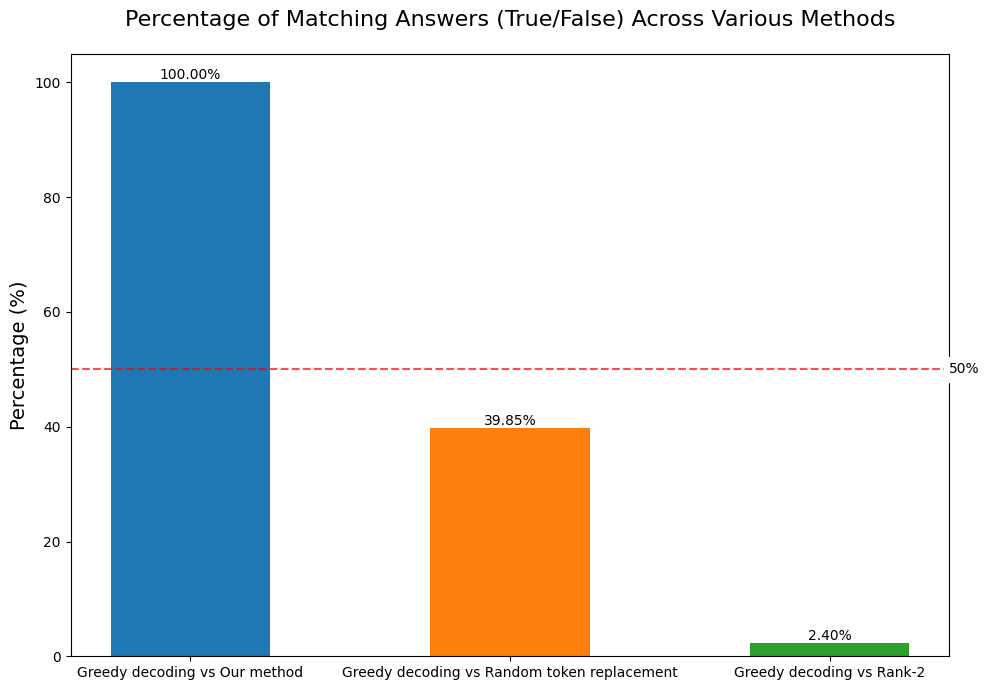
\includegraphics[width=\textwidth]{token_comparison_percentages.png}
\caption{Comparison of decoding methods}
\label{fig:decoding_comparison}
\end{figure}

\section{Implications and Future Work}
Our findings provide new tools for understanding internal reasoning processes and increase confidence in COT-based approaches for improving visibility. Future work should focus on developing better decoding methods or finding circuits that hide tokens, investigating generalizability to tasks beyond 3SUM (including natural language tasks), and improving token hiding methods (currently limited to one hidden token which is simple to decode).


\clearpage
\section{Conclusion}
We have presented a novel approach to understanding hidden computations in transformer models through analysis of token rankings and layer-wise representations, and development of a modified decoding algorithm. Our insights into how models encode and process information in hidden COT sequences open new avenues for improving interpretability, efficiency, and safety in language models. This work strengthens the belief in COT visibility research for interpretability.

\appendix
\begin{figure}[p]
    \centering
    \section{Layerwise comparison of decoding methods}
    \vspace{-0.5em}  % Reduce space after the title
    
    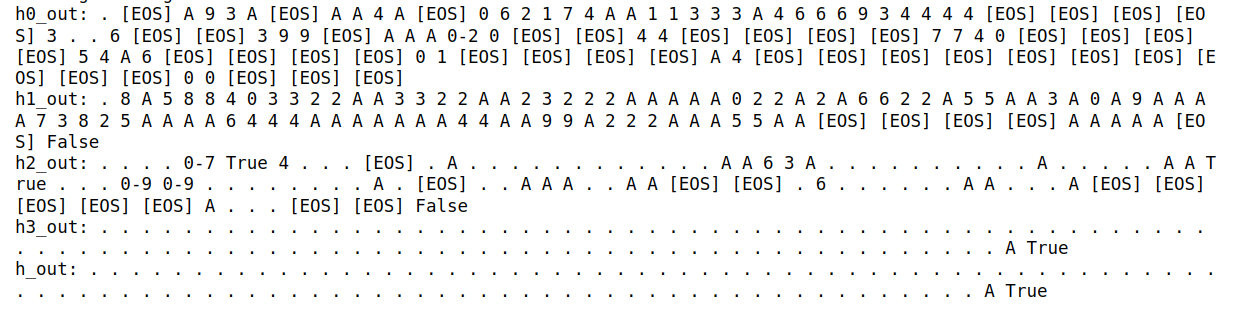
\includegraphics[width=\textwidth,height=0.19\textheight,keepaspectratio]{greedy_decoding.png}
    \captionof{figure}{Greedy Decoding}
    \label{fig:greedy}
    
    \vspace{0.5em}
    
    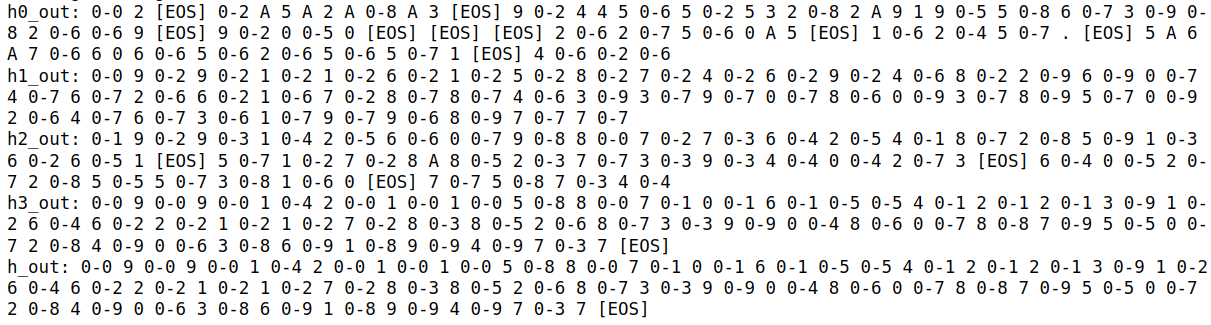
\includegraphics[width=\textwidth,height=0.19\textheight,keepaspectratio]{rank2_decoding.png}
    \captionof{figure}{Greedy Decoding with Rank-2 Tokens}
    \label{fig:rank2}
    
    \vspace{0.5em}
    
    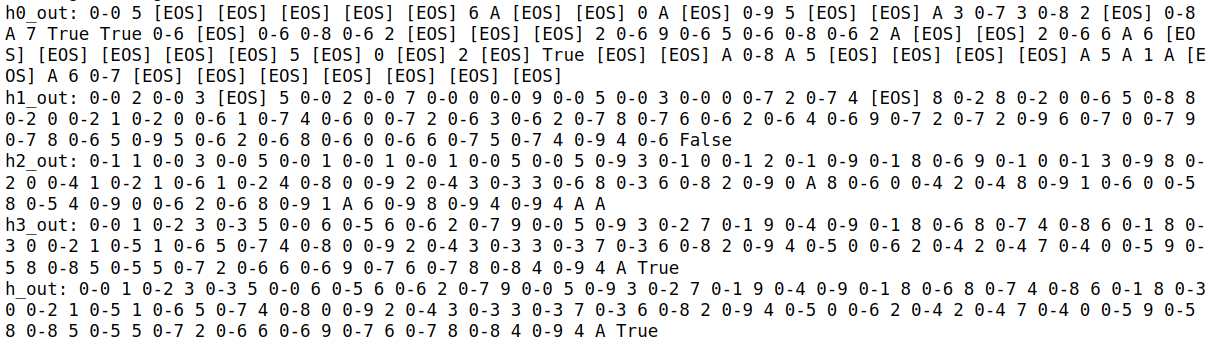
\includegraphics[width=\textwidth,height=0.19\textheight,keepaspectratio]{our_method_decoding.png}
    \captionof{figure}{Our Method: Greedy Decoding with Hidden Tokens Replaced by Rank-2 Tokens}
    \label{fig:our-method}
    
    \vspace{0.5em}
    
    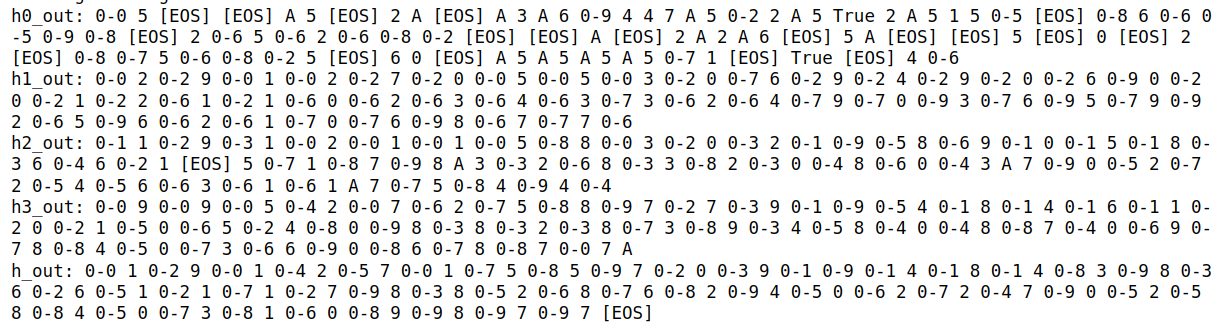
\includegraphics[width=\textwidth,height=0.19\textheight,keepaspectratio]{random_tokens_decoding.png}
    \captionof{figure}{Greedy Decoding with Hidden Tokens Replaced by Randomly Selected Tokens}
    \label{fig:random}
\end{figure}
\end{document}
